\documentclass[10pt,addpoints]{exam}
\usepackage[utf8]{inputenc}
\usepackage[spanish,es-noshorthands]{babel}
\usepackage{hyperref}
\usepackage{amsmath}
\usepackage{amsfonts}
\usepackage{amssymb}
\usepackage{graphicx}
\usepackage{mathrsfs}
\usepackage{tikz}
\usepackage{multicol}
\usepackage[papersize={6.5in,8.5in},top=.75cm,right=.75cm,left=.75cm,bottom=.75cm]{geometry}
\printanswers
\begin{document}
\title{\begin{minipage}{.2\textwidth}
        
\includegraphics[height=1.75cm]{Images/logo-colegio.png}
       \end{minipage}
\begin{minipage}{.55\textwidth}
 \begin{center}
Prueba Saber $5^{\circ}$ de primaria\\Matemáticas $9^{\circ}$
\end{center}
\end{minipage}
\begin{minipage}{.2\textwidth}

\includegraphics[height=1.75cm]{Images/logo-sed.png} 
\end{minipage}
}
\author{Germ\'{a}n Avendaño Ram\'{i}rez~\thanks{Lic. Mat. U.D., M.Sc. U.N.}}
\date{}
\maketitle
\begin{center}
\fbox{\fbox{\parbox{5.5in}{\centering
Conteste en el cuadro de respuestas diseñado para tal fin. Puede usar una hoja en blanco para hacer operaciones. \emph{Prohibido el uso de la calculadora o cualquier dispositivo electrónico}}}}
\end{center}
Formulario \textbf{A}
\begin{multicols}{2}
\begin{questions}
\question Con bloques de madera iguales, se construyó una torre como la que se muestra en la siguiente figura:
\begin{center}
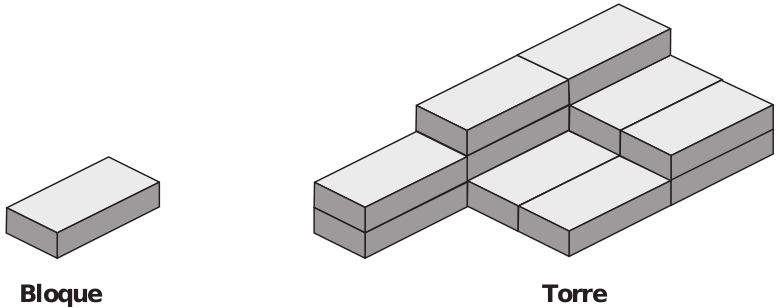
\includegraphics[scale=.2]{Images/Pantallazo-15.png} 
\end{center}
¿Con cuántos bloques se formó la torre?

\begin{oneparchoices}
\choice 7
\choice 8
\choice 10
\CorrectChoice 14
\end{oneparchoices}
\question
La siguiente gráfica muestra los puntajes obtenidos por unos jugadores, luego de lanzar varias veces dos dados y sumar los puntos de sus caras superiores.
\begin{center}
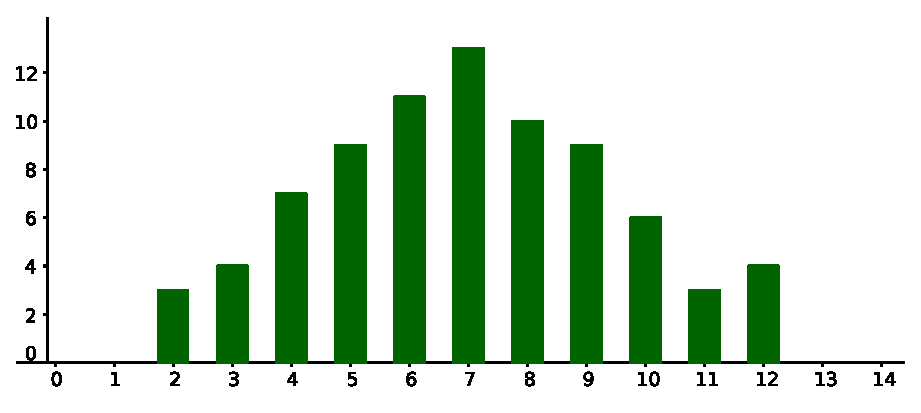
\includegraphics[scale=.55]{Images/diag-barras.eps} 
\end{center}
¿Cuál de las siguientes afirmaciones es verdadera?
\begin{choices}
\choice Los puntajes que salieron menos veces fueron el 5, el 9 y el 10.
\CorrectChoice Los puntajes que salieron más veces fueron el 6, el 7 y el 8.
\choice El puntaje que salió menos veces fue el 12.
\choice El puntaje que salió más veces fue el 4.
\end{choices}
Responda las preguntas \ref{q01}--\ref{q02} de acuerdo con la siguiente información

Una papelería ofrece la siguiente promoción:
\begin{center}
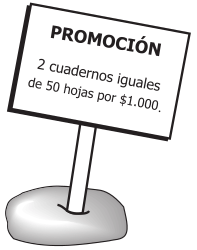
\includegraphics[scale=.5]{Images/Pantallazo-17.png} 
\end{center}
\question \label{q01}
Con \$8.000, ¿cuántos cuadernos de la promoción se puede comprar sin que sobre dinero?

\begin{oneparchoices}
\choice 4
\choice 8
\choice 12
\CorrectChoice 16
\end{oneparchoices}
\question \label{q02}
¿En cuál de las siguientes tablas se muestra el precio correcto de 2, 4, 6 y 8 cuadernos iguales de 50 hojas?

\begin{choices}
\choice \begin{tabular}{|c|c|}
\hline 
\# cuadernos & Precio (\$) \\ 
\hline 
2 & 1000 \\ 
\hline 
4 & 2000 \\ 
\hline 
6 & 4000 \\ 
\hline 
8 & 8000 \\ 
\hline 
\end{tabular}
\choice \begin{tabular}{|c|c|}
\hline 
\# cuadernos & Precio (\$) \\ 
\hline 
2 & 500 \\ 
\hline 
4 & 1000 \\ 
\hline 
6 & 1500 \\ 
\hline 
8 & 2000 \\ 
\hline 
\end{tabular} 
\choice \begin{tabular}{|c|c|}
\hline 
\# cuadernos & Precio (\$) \\ 
\hline 
2 & 500 \\ 
\hline 
4 & 1000 \\ 
\hline 
6 & 2000 \\ 
\hline 
8 & 3000 \\ 
\hline 
\end{tabular} 
\CorrectChoice \begin{tabular}{|c|c|}
\hline 
\# cuadernos & Precio (\$) \\ 
\hline 
2 & 1000 \\ 
\hline 
4 & 2000 \\ 
\hline 
6 & 3000 \\ 
\hline 
8 & 4000 \\ 
\hline 
\end{tabular} 
\end{choices}
\question Pedro tenía algunos dulces guardados, se comió la mitad y regaló 2. Ahora tiene 4 dulces. ¿Cuántos dulces tenía guardados Pedro?

\begin{oneparchoices}
\choice 6
\choice 8
\choice 10
\CorrectChoice 12
\end{oneparchoices}
\question Para elaborar una tarjeta de felicitación, Marta dobló una hoja de papel por la mitad, como se indica a continuación:
\begin{center}
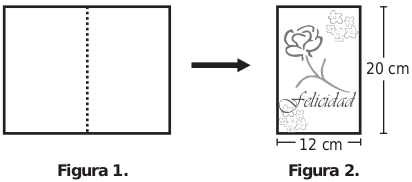
\includegraphics[scale=.5]{Images/Pantallazo-19.png} 
\end{center}
La tarjeta tiene las medidas indicadas en la figura 2.
¿Cuáles son las medidas de los lados de la hoja que Marta dobló?
\begin{choices}
\choice 10 y 6 cm
\CorrectChoice 20 y 24 cm
\choice 20 y 6 cm
\choice 10 y 12 cm
\end{choices}
RESPONDE LAS PREGUNTAS 21 Y 22 DE ACUERDO CON LA SIGUIENTE INFORMACIÓN

Claudia compró varios metros de cinta, unos de color amarillo y otros de color azul.
\question Con 15 metros de cinta amarilla, Claudia puede hacer 5 adornos del mismo tamaño, iguales, sin que sobre cinta. ¿Cuántos adornos del mismo tamaño de los amarillos puede hacer con 30 metros de cinta azul sin que sobre cinta?

\begin{oneparchoices}
\choice 3
\choice 5
\CorrectChoice 10
\choice 15
\end{oneparchoices}
\question Claudia tomó 12 metros de cinta amarilla y 20 metros de cinta azul y los cortó de forma que resultaran pedazos del mismo tamaño, no sobrara cinta y fueran de la mayor longitud posible. ¿Cuál es la longitud de cada pedazo?
\begin{choices}
\choice 3 metros
\CorrectChoice 4 metros
\choice 5 metros
\choice 6 metros
\end{choices}
RESPONDE LAS PREGUNTAS 41 Y 42 DE ACUERDO CON LA SIGUIENTE INFORMACIÓN

En una finca hay 600 animales distribuidos en dos zonas, zona A y zona B . De los 600 animales, $\frac{4}{6}$ está en la zona A y el resto de los animales esta en la zona B.
\question ¿Cuál diagrama representa correctamente la distribución de los animales en las dos zonas?
\begin{center}
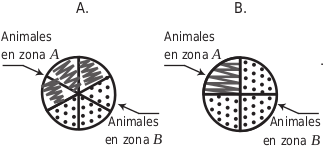
\includegraphics[scale=.5]{Images/Pantallazo-21.png}
\end{center}
\begin{center}
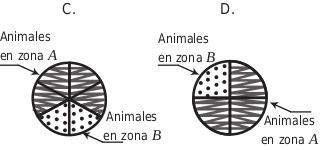
\includegraphics[scale=.5]{Images/Pantallazo-22.png} 
\end{center}
\question Si $\frac{1}{4}$ de los animales que estaba en la zona A pasó a la zona B , ¿Cuántos animales están ahora en la zona B ?

\begin{oneparchoices}
\choice 100
\choice 150
\CorrectChoice 300
\choice 400
\end{oneparchoices}
\question Un número es divisible por 3 si al sumar sus cifras resulta un múltiplo de 3. Por ejemplo, 219, 48 y 12 son números divisibles por 3.

171 es divisible por 3 porque:
\begin{choices}
\choice 171 es un número primo
\choice 171 es un número impar
\choice $1 \times 7 \times 1$ es múltiplo de 3
\CorrectChoice $1+7+1$ es múltiplo de 3
\end{choices}
\question La profesora Diana les preguntó a 60 estudiantes de grado cuarto cuál de los siguientes libros preferían leer:
\begin{itemize}
\item Zoro
\item La isla del tesoro
\item Harry Potter
\item Cuentos de los hermanos Grimm
\end{itemize}
Con las respuestas obtenidas, la profesora Diana elaboró la siguiente gráfica:
\begin{center}
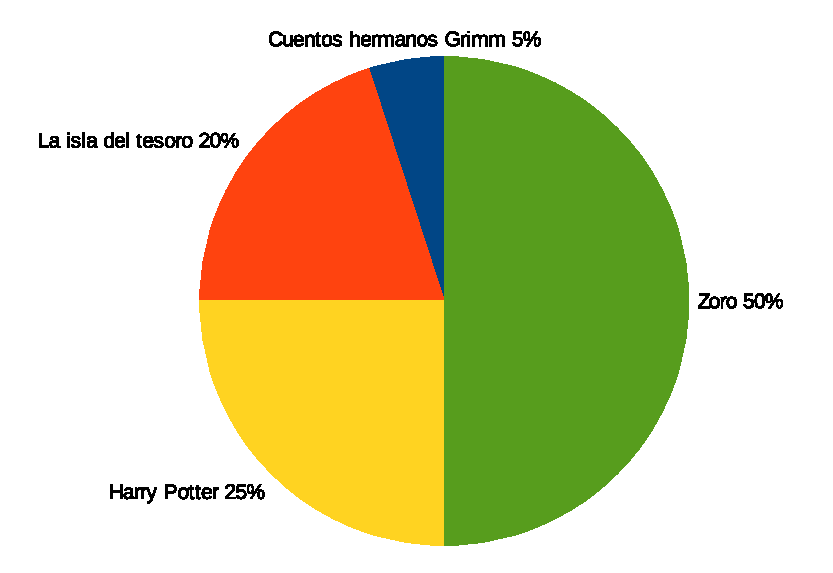
\includegraphics[scale=.5]{Images/Pantallazo-23.eps} 
\end{center}
En la clase se leerán los libros escogidos por más de 10 estudiantes. ¿Cuáles son estos libros?
\begin{choices}
\choice Zoro solamente
\choice Zoro y La isla del tesoro solamente
\CorrectChoice Zoro, Harry Potter y La isla del tesoro solamente
\choice Zoro, Harry Potter, La isla del tesoro y Cuentos de los hermanos Grimm
\end{choices}
\question La figura que se muestra a continuación se debe construir usando piezas.
\begin{center}
\begin{tikzpicture}[scale=1.75]
\draw (0,0)--node[below]{15cm}(1.5,0)--node[right]{5cm}(1.5,0.5)--node[above]{10cm}(0.5,0.5)--(0.5,1)--(0,1)--node[left]{10cm}cycle;
\end{tikzpicture}
\end{center}
Se dispone de los siguientes grupos de piezas:
\begin{enumerate}
\item[I.] \fbox{\tikz[scale=.75] \draw (0,0)--node[below]{5cm}(1,0)--(1,2)--(0,2)--node[left]{10cm}cycle; \; \tikz[scale=.75] \draw (0,0)--node[below]{5cm}(1,0)--node[right]{10cm}(1,2)--cycle;}
\item[II.] \fbox{\tikz[scale=.75] \draw (0,0)--node[below]{5cm} (1,0)--node[right]{10cm}(1,2)--(0,2)--cycle; \; \tikz[scale=.75] \draw (0,0)--node[below]{5cm} (1,0)--node[right]{10cm}(1,2)--(0,2)--cycle;}
\item[III.] \tikz[scale=.75] \draw (0,0)--node[below]{5cm}(1,0)--(0,2)--node[left]{10cm}(0,0); \; \tikz[scale=.75] \draw (0,0)--node[left]{5cm}(0,1)--(2,0)--node[below]{10cm}(0,0);\;
\tikz[scale=.75] \draw (0,0)--node[below]{10cm}(2,0)--node[right]{5cm}(2,1)--cycle; \tikz[scale=.75] \draw[rotate around={40:(0,0)}] (0,0)--node[below]{5cm}(1,0)--(1,2)--node[left]{10cm}cycle;
\end{enumerate}
La figura se puede construir utilizando las piezas del(os) grupo(s)
\begin{choices}
\choice I solamente
\choice I y II solamente
\CorrectChoice II y III solamente
\choice III solamente
\end{choices}
\question Para la fiesta de cumpleaños de Valeria se preparó una torta y se partió en 10 porciones iguales.

Valeria se comió $\frac{3}{10}$ de su torta de cumpleaños.

¿En cuál de las siguientes gráficas se representan las porciones de torta que se comió Valeria?
\begin{choices}
\choice 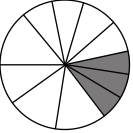
\includegraphics[scale=.5]{Images/Pantallazo-24.png} 
\choice 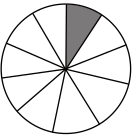
\includegraphics[scale=.5]{Images/Pantallazo-25.png} 
\CorrectChoice 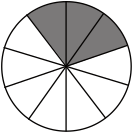
\includegraphics[scale=.5]{Images/Pantallazo-26.png} 
\choice 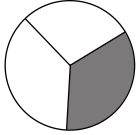
\includegraphics[scale=.5]{Images/Pantallazo-27.png} 
\end{choices}
\question Un examen de quinto de primaria contenía preguntas en tres áreas: Matemáticas, Ciencias Naturales y Lenguaje. En la tabla se muestra el número de preguntas en el examen por cada área. En la gráfica 1 se muestra la cantidad de respuestas correctas de algunos de los estudiantes que contestaron el examen.

\begin{tabular}{|c|c|}
\hline 
Materia & Número de preguntas \\ 
\hline 
Matemáticas & 30 \\ 
\hline 
C. Naturales & 35 \\ 
\hline 
Lenguaje & 25 \\ 
\hline 
\end{tabular}
\begin{center}
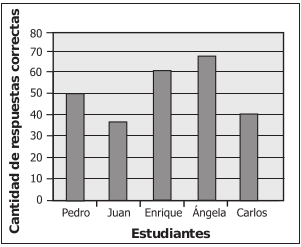
\includegraphics[scale=.6]{Images/Pantallazo-18.png} 
\end{center}
De los estudiantes que se muestan en la gráfica, ¿quiénes contestaron correctamente más de la mitad de las preguntas del examen?
\begin{choices}
\choice Juan y Carlos, solamente.
\choice Enrique y Ángela, solamente.
\choice Pedro, Juan y Carlos, solamente.
\CorrectChoice Pedro, Enrique y Ángela, solamente.
\end{choices}
\end{questions}
\end{multicols}
\end{document}
